\documentclass[conference]{IEEEtran}

%% DOCUMENT FORMATTING
\usepackage[ngerman]{babel}
\usepackage{csquotes}
\usepackage{geometry}

%% Hyperlinks
\usepackage{hyperref}

%% GRAPHICS
\usepackage{graphicx}

% Math Shit
\usepackage{amsmath}
\usepackage{physics} % http://mirrors.ibiblio.org/CTAN/macros/latex/contrib/physics/physics.pdf

% CITATION
\usepackage{acronym}

% MATH

\usepackage{physics}

\usepackage[style=ieee, maxcitenames=2, mincitenames=1]{biblatex}
\addbibresource{sources.bib}


\def\BibTeX{{\rm B\kern-.05em{\sc i\kern-.025em b}\kern-.08em
    T\kern-.1667em\lower.7ex\hbox{E}\kern-.125emX}}
\begin{document}
\pagenumbering{Roman} 

\title{Post Quanten Kryptographie\\
\large \ \\ \large Warum wir schon jetzt neue Verschlüsselungsalgorithmen brauchen}

\author{
  \IEEEauthorblockN{Thomas Jakkel}
  \IEEEauthorblockA{\textit{MatNr. 1001594} \\
  01jath1bif@hft-stuttgart.de}

  \and

  \IEEEauthorblockN{Lukas Reinke}
  \IEEEauthorblockA{\textit{MatNr. 1001213} \\
  01relu1bif@hft-stuttgart.de}
}

\maketitle

\begin{abstract}
    Quantenkryptographie wird als ernsthafte Gefahr für die aktuell gängigen Kryptographie-Verfahren gesehen. Speziell die, für das sichere Funktionieren der Netzwerk-Kommunikation benötigten, asymmetrischen Kryptographie-Algorithmen wie beispielsweise \textit{RSA} stehen in der Gefahr mithilfe eines Quantencomputers innerhalb von Stunden gebrochen zu werden. Ein solcher Computer birgt somit eine Gefahr für die gesamte heutige Informationssicherheit.\\
    Schon 1994 bewies der amerikanische Mathematiker \textit{Peter Shor} in der Theorie, wie mithilfe eines Quantencomputers die Primfaktorzerlegung großer Zahlen in realer Zeit erfolgen kann. Mit einem klassischen, binären Computer wäre dies nicht in der Lebenszeit des Universums möglich, was zentrale Sicherheits-Prinzip asymmetrischer Kryptographie darstellt.
    Wegen dieser Bedenken hat das US National Institute of Standards and Technology (NIST) seit 2016 eine Ausschreibung zur Entwicklung eines quantensicheren Algorithmus aufgestellt. Der aktuelle Favorit, ein Verfahren auf basis mehrdimensionaler Vektorfelder, soll, soweit sich keine Schwachstellen herausstellen, schon in den nächsten Jahren in der Netzwerk Kryptographie etabliert werden und somit die Kommunikation schon vor der Existenz eines potentiellen Quantencomputers absichern. Es ist also gut möglich, dass wir die aktuellen Kryptographie Standards innerhalb der nächsten 5 Jahre austauschen werden.
\end{abstract}

\listoffigures
\addcontentsline{toc}{section}{Abbildungsverzeichniss}

\section*{Abkürzungsverzeichnis}
\begin{acronym}
  \acro{qc}[QC]{Quantencomputer}
\end{acronym}

\section{Einleitung}
Das Thema der \textit{Quanten Supremacy}, der Zeitpunkt zu dem ein \ac{qc} die Fähigkeit besitzt komplexe Probleme besser zu lösen als ein klassischer Computer, ist in den letzten Jahren immer wieder in einschlägigen Medien und diverse Fachpublikationen aufgetaucht. Google zum Beispiel behauptete schon wiederholt einen solchen \ac{qc} zu besitzen, was jedoch in diversen Publikationen bezweifelt wurde \cite{cho_ordinary_2022}. Wenig Zweifel besteht jedoch, dass ein solcher Computer in absehbarer Zeit einsatzbereit sein wird.\\ 
%% mabybe number of qubits to usability? 
Im Folgenden wird beschieden wie ein \ac{qc} funktioniert, mit welchen Algorithmen, die in realer Zeit laufen, \ac{qc} die aktuellen, kryptographischen Verfahren brechen können werden. Außerdem werden wir aktuelle, neu Entwickelte quantensichere Algorithmen betrachten und wie sie sie Gefahr durch \ac{qc} mittigern werden.

\section{Einführung in das Quanten Computing}
Quanten Computing ist eine relativ junge Disziplin der Physik und Informatik. Obwohl die Entwicklung der beiden Bereiche unabhängig voneinander zu Beginn des 20. Jahrhunderts begann, wurden schon in den 1980er Jahren die ersten Versuche unternommen und theoretische Überlegungen angestellt, um Methoden der Informatik mithilfe von Quantenobjekten umzusetzen. Obwohl der \ac{qc} erst seit kurzer Zeit existiert, hat er bereits bedeutende Fortschritte gemacht und besitzt ein enormes Potenzial für Entwicklungen zum Beispiel in den Bereichen Kryptographie, Optimierungsprobleme, Simulation chemischer Prozesse und maschinelles Lernen.

\subsection{Ein theoretischer Quantencomputer}
Ein der Informatik zugrunde liegendes Prinzip ist, dass \cite[S122]{steane_quantum_1998} Informationen auf unterschiedlichen Weisen dargestellt (codiert) werden können. So kann die Zahl \textit{fünf} zum Beispiel binär ($0101$) oder als Unicode Zeichen (\textit{U+0035}) dargestellt werden. Der Inhalt der Information ist in beiden Fällen jedoch der Gleiche.\\
Dieses Prinzip ist für die Informatik sehr wichtig. Es ermöglicht Maschinen komplexe Informationen zu speichern, mithilfe einfacher Operationen zu manipulieren und wieder in ein komplexes Format zu überführen, ohne dabei an Informationsgehalt zu verlieren oder Informationen unkenntlich zu machen. In einem Computer werden diese Informationen in Form von \textit{bits} darstellt die zwei Zustände, repräsentiert durch \textit{0} und \textit{1}, annehmen können. In einem klassischen, digitalen Computer sind diese beispielsweise durch das fließen von Strom abgebildet. Ein \ac{qc} repräsentiert Informationen in den Eigenschaften von Quanten-Objekten, beispielsweise dem Spin von Elektronen.\\
%% Universaler \ac{qc} ???
Um die Funktion eines \ac{qc} zu erläutern muss erst ein kurzer Blick auf einige quantenphysikalische Phänomene geworfen werden.

\subsubsection{Superpositionen}
Eine Superposition ist das Fundamentale quantenphysische Phänomen das einem \ac{qc} zugrunde Liegt.
Es wird meistens mithilfe des Gedankenexperiments von \cite[\$5]{schrodinger_gegenwartige_1935} \textit{Schrödingers Katze} veranschaulicht: In einer Box befindet sich eine Katze und ein Gefäß mit Gift das zerstört wird und die Katze tötet, wenn ein radioaktiver Zerfall gemessen wird. Außerhalb der Box lässt sich nicht feststellen, ob der Mechanismus der das Gift freisetzt aktiviert wurde. Sie befindet sich, Quantenmechanisch gesehen, in einem Zustand in dem sie sowohl tot als auch lebendig ist. In dem Moment, in dem die Box geöffnet wird, kann festgestellt werden welcher der beiden Zustände eingetroffen ist.\\
Auf ein \ac{qt} übertragen heißt das: Es kann sich in einem undefinierten Zustand befinden, der \textbf{Superposition} aus allen möglichen Zuständen. Erst wenn \textit{nachgeschaut}, also der Zustand gemessen wird, kollabiert die Superposition in einen der möglichen Zustände. Eine Superposition kann durch die Wahrscheinlichkeit, mit der jeder der Zustände eintreten kann, beschrieben werden. Ein Elektron mit den Zuständen Spin up ($75\%$) und Spin down ($25\%$) kollabiert also, wenn der Spin gemessen wird zu $3/4$ der Fälle als Spin up und zu $1/4$ als Spin down.
Mathematisch kann eine Superposition $\psi$ als Linearkombination ihrer Zustände betrachtet werden. 
\begin{equation}
    \ket{\psi } = \alpha \ket{1} + \beta \ket{0} \\
\end{equation}
Diese Linearkombination kann auch grafisch, als Vektor auf einer Kugel dargestellt werden (siehe Graphik \ref{fig:spin}). Es ist zu beachten, dass der Vektor \textit{z} nicht den Spin, sondern die Linearkombination darstellt.

\begin{figure}[!hbt]
    \centering
    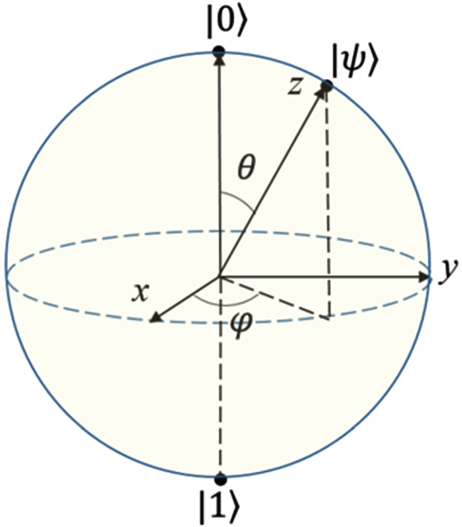
\includegraphics{./images/spin-superpostition.jpg}
    \caption{Spin eines Elektrons in Superposition \cite{noauthor_cpb_27_9_090308_f8jpg_nodate}}
    \label{fig:spin}
\end{figure}

\subsubsection{Quantenverschränkung}
Das zweite quantenphysikalische Phänomen auf dem ein Quantencomputer basiert ist die \textbf{Quantenverschränkung}. Der Zustand verschränkter \ac{qt} is voneinander abhängig. Verändert sich der Zustand eines einzelnen \ac{qt}s Verändert sich der Zustand aller mit ihm verschränken \ac{qt}. Das bedeutet auch: Wird der Zustand eines \ac{qt}s gemessen und seine die Superposition kollabiert, so kollabiert die Superposition aller verschränken \ac{qt} \cite{miller_principles_nodate}.\\

\subsection{Implementierung eines Quantencomputers}

Mit den oben erläuterten Phänomenen sind wir nun in der Lage einen Quantencomputer zu konstruieren. Ein klassischer Computer kann in einem Bit immer nur eine Information auf ein mal darstellen. In zwei bit kann somit eine der Kombinationen aus dem Folgenden Set darstellen.

\begin{equation}
    Klassischer Computer: \{00, 01, 10, 11\}
\end{equation}

Ein \ac{qc} hingegen kann mithilfe verschränkter \ac{qt} das Set aus allen Möglichen Informationen repräsentieren.

\begin{equation}
    Quantencomputer: \ket{\psi_0 \psi_1} 
\end{equation}

Was alle Elemente aus dem folgenden Set repräsentiert.

\begin{equation}
    \{ \ket{00}, \ket{01}, \ket{10}, \ket{11} \}
\end{equation} \cite[142]{steane_quantum_1998}

Die Herausforderung ist nun die richtige Lösung aus der Menge aller möglicher Lösungen heraus zu extrahieren. Messen wir den Zustand eines \ac{qt} so kollabieren die verschränken Superpositionen zu einer der möglichen Informationen, alle Informationen können nicht auf ein mal ausgelesen werden. Auch ist es nicht möglich ein mal gemessene \ac{qt}s wieder in eine Superposition zu versetzen. Wie ist es nun möglich mit einem \ac{qc} Berechnungen anzustellen?

\subsubsection{Quantenregister}
Ein \ac{qr} ist ein grundlegender Bestandteil eines \ac{qc} und repräsentiert den Speicher für Quanteninformationen. Es ist vergleichbar mit einem klassischen Register in einem herkömmlichen Computer.

Ein \ac{qr} besteht aus einer Anordnung von Qubits und dient als Container, um diese zu speichern und sie miteinander zu manipulieren. Die Anzahl der Qubits in einem \ac{qr} bestimmt die Größe und Komplexität der Berechnungen, die ein \ac{qc} durchführen kann. Je größer das \ac{qr} ist, desto mehr Qubits stehen zur Verfügung, um komplexe Berechnungen durchzuführen.

Durch die Anwendung von Quantengattern, wie beispielsweise Hadamard-Gattern, CNOT-Gattern und Phasengattern, können Operationen auf den Qubits im \ac{qr} ausgeführt werden. Diese Gatter ermöglichen es, Qubits zu verschränken, Superpositionen zu erzeugen und gezielte Manipulationen der Quanteninformationen durchzuführen.

Das \ac{qr} spielt eine zentrale Rolle in Quantenalgorithmen, da es die Plattform bietet, auf der die Quantenberechnungen durchgeführt werden. Die Größe und Qualität des \ac{qr}s sind entscheidend für die Leistungsfähigkeit eines Quantencomputers. Daher ist die Entwicklung und Skalierung von \ac{qr}n ein aktiver Bereich der Forschung, um die Möglichkeiten der Quantencomputertechnologie weiter zu verbessern.

%Quellen:
%[1] Nielsen, M. A., & Chuang, I. L. (2010). Quantum Computation and Quantum Information. Cambridge University %Press.
%[2] Mermin, N. D. (2007). Quantum Computer Science: An Introduction. Cambridge University Press.
%[3] Kaye, P., Laflamme, R., & Mosca, M. (2007). An Introduction to Quantum Computing. Oxford University Press.

\subsection{Fehlerkorrektur}

\section{RSA}
\input{chapters/04_RSA.tex}

\section{Shors-Algorithmus}
% Einleitung Primfaktorzerlegung\\
Die Faktorisierung großer Zahlen \cite[S189]{bernstein_post-quantum_2017} ist ein fundamentales mathematisches Problem, 
bei dem eine gegebene Zahl in ihre Primfaktoren zerlegt wird.
Dieses Problem ist von zentraler Bedeutung für die Kryptographie, da viele asymmetrische Verschlüsselungsverfahren, wie beispielsweise RSA, 
auf der Schwierigkeit der Faktorisierung großer Zahlen beruhen.

Das Problem der Primfaktorzerlegung besteht darin, eine öffentliche Zahl $N$ in zwei oder mehr geheime Primzahlen $p$ und $q$ zu zerlegen, sodass: $N = p*q$. 
Für kleine Zahlen kann die Faktorisierung durch Ausprobieren möglicher Primfaktoren relativ einfach sein. 
Allerdings wird die Faktorisierung bei großen Zahlen exponentiell schwieriger, 
da es keine effizienten klassischen Algorithmen gibt, welche dies in Polynomialzeit bewältigen können.

Die Sicherheit vieler asymmetrischer Verschlüsselungsverfahren, 
wie beispielsweise das RSA-Verfahren, beruht auf der Schwierigkeit der Faktorisierung großer Zahlen. 
Wenn ein Angreifer in der Lage wäre, die Primfaktoren einer Zahl zu finden, 
könnte er den geheimen Schlüssel einer Verschlüsselungsmethode berechnen und die Sicherheit des Systems kompromittieren.\\

% Shors Algorithmus
Shors Algorithmus \cite{shor_algorithms_1994} gilt als einer der bedeutendsten Quantenalgorithmen, 
der die Faktorisierung großer Zahlen in Polynomialzeit ermöglicht. 
Auch wenn dieser Algorithmus einen \ac{qc} mit vielen, stabilen Qubits voraussetzt, 
stellt diese revolutionäre Entdeckung bereits heute eine enorme Bedrohung für die moderne Kryptographie dar.
Zum einen wird effektiv an \ac{qc} geforscht, die Anzahl stabiler Qubits in \ac{qc} steigen. 
Wenn der \ac{qc} seinen Durchbruch in unserer Gsellschaft erreicht hat, müssen wir darauf vorbereitet sein und uns bereits heute mit den Konsequenzen auseinander setzen. 
Zum anderen werden verschlüsselten Daten bereits heute gespeichert, um sie in der Zukunft entschlüsseln zu können und 
im Nachinein an wichtige, vertrauliche Informationen zu gelangen. In der Kryptographie spricht man von dem Prinzip: \glqq Safe now, decrypt later\grqq.\\

Im folgenden \cite{kak_lecture_nodate}\cite[S. 4-5]{gidney_how_2021} werden wir an einem vereinfachten Beispiel näher aufzeigen, 
wie Shors Algorithmus eine effiziente Lösung für die Faktorisierung großer Zahlen auf einem \ac{qc} bietet.
Zunächst betrachten wir die öffentliche Zahl $N$, welche in ihre Primfaktoren $p$ und $q$ zerlegt werden soll. 
Für das vereinfachte Beispiel wählen wir $N = 77$. Also: $$N = p*q \textrm{ mit } N= 77$$
\textit{Beachte das $N$ in Realität eine riesige Zahl ist. Das vereinfachte Beispiel soll ledeglich den Prozess von Shors Algorithmus aufzeigen}.

Nun stellen wir eine zweite Gleichung 
$${g^r = mN+1}$$ 
auf, welche behauptet, dass man immer einen Exponenten $r$ finden kann, sodass ein Vielfaches einer zufälligen Zahl $g < N$ gleich einem vielfachen $m$ der Zahl $N+1$ ist.
Wir wählen zufällig die Zahl $g = 8$ und erhalten aus Abbildung \ref{fig:Zufallszahl $g^x$ mit Rest} $r = 10$

\begin{figure}[h]
    \begin{center}
        \begin{tabular}{|c|c|c|} \hline
            $g^x$       &   $g^x/77$    &   Rest    \\\hline
            $g^0$       &   0           &   1       \\\hline
            $g^1$       &   0           &   8       \\\hline
            $g^2$       &   0           &   64      \\\hline
            $g^3$       &   6           &   50      \\\hline
            $g^4$       &   53          &   15      \\\hline
            $g^5$       &   425         &   43      \\\hline
            $g^6$       &   3404        &   36      \\\hline
            $g^7$       &   27235       &   57      \\\hline
            $g^8$       &   217885      &   71      \\\hline
            $g^9$       &   1733087     &   29      \\\hline
            $g^{10}$    &   13944699    &   1       \\\hline
        \end{tabular}\\
    \end{center}
    \caption{Zufallszahl $g^x$ mit Rest}
    \label{fig:Zufallszahl $g^x$ mit Rest}
\end{figure}

Wie extrahiert man aus der Funktion $g^{10} = mN + 1$ die Primfaktoren $p, q$? Hierfür schreiben wir unsere ursprüngliche Gleichung um und erhalten:

\begin{align*}
                        &   g^r = mN+1      \\
    \Leftrightarrow\;\; &   g^r - 1 = mN    \\
    \Leftrightarrow\;\; &   g^r - 1 = mN    \\
    \Leftrightarrow\;\; &   (g^{r/2} + 1)(g^{r/2} - 1) = mN
\end{align*}

Mit $r = 10$ erhalten wir:

\begin{align*}
    (g^{r/2} + 1) &= (8^5 + 1) &= 32.769 \\
    (g^{r/2} - 1) &= (8^5 - 1) &= 32.767
\end{align*}

Damit haben wir aus einer geschätzten Zahl $g = 8$ zwei Zahlen gefunden, welche vermutlich Faktoren mit $N$ teilen. 
Um diese Faktoren zu finden, wenden wir den euklidischen Algorithmus an, um den \ac*{ggT} zu finden:

\begin{align*}
    & 32.769 / 77 &=\;&  425 R 44    \\
    & 77 / 44     &=\;&  1 R 33      \\
    & 44 / 33     &=\;&  1 R 11      \\
    & 33 / 11     &=\;&  3 R 0       \\
    \Rightarrow\;\; & ggT(32.769, 77) = 11
\end{align*}

Wir erhalten somit als ersten Faktor $p = 11$. 
Für den zweiten Faktor kann der selbe Prozess nochmals mit der zweiten Zahl berechnet werden, oder wir erhalten durch $q = N/p \Leftrightarrow q = 7$. 
Damit haben wir erfolgreich die Zahl $N = 77$ in ihre Primfaktoren $p=11$ und $q=7$ zerteilt.\\


Nachfolgend fassen wir nochmal die Schritte zusammen, wie man eine eine öffentliche Zahl $N$, ein Produkt aus zwei Primzahlen faktorisiert.

\begin{enumerate}
    \item Schätze eine Zahl $g < N$
    \item Finde einen Exponenten $r$ sodass\\$g^r = mN + 1$
    \item Berechne $(g^{r/2} + 1)$ und $(g^{r/2} - 1)$
    \item Nutze den euklidischen Algorithmus um den \ac{ggT} zu finden\\
\end{enumerate}

Um diesen Algorithmus auszuführen bräuchte es noch keinen \ac{qc}, jedoch wäre diese Methode auf einem klassischen Computer nicht schneller, als herkömmliche Methoden. 
Der Kernprozess, welcher ein \ac{qc} beschleunigt ist Schritt 2. Um dies zu verstehen, betrachten wir Abbildung \ref{fig:Zufallszahl $g^x$ mit Rest} nochmal genauer. 
Würde man die Tabelle fortführen, würde sich der Restanteil der Zahlen stets wiederholen. In unserem obrigen Beispiel mit der Periode $10$, 
wie sich aus $g^0 Rest 1$ und $g^{10} Rest 1$ erkennen lässt. Dies gilt ebenfalls für die anderen Zahlen, beispielsweise würde $8^{13} Rest 50$ haben.
Dies bedeutet, dass sich Schritt 2 beschleunigen lässt indem man die Periode findet, mit der sich der Restanteil wiederholt. 
An dieser Stelle setzt der Quantenpart ein.\\

% Quanten Part
Für die Quantenberechnung \cite[S.1-2]{amico_experimental_2019} werden zwei \ac{qr} benötigt. Ein Periodenregister $n_p$, 
um den Wert der Periode zu speichern und ein Ergebnisregister $n_q$ um das Ergebnis der Berechnung zu speichern. 
Die Größe der beiden Register hängt von der Zahl $N$ ab, welche faktorisiert werden soll. 
Das Periodenregister benötigt eine Anzahl von Qubits $n_p$, von etwa $\log_2(N^2) \le n_p \le log_2(2N^2)$. 
Das Ergebnisregister muss ledeglich groß genug sein, um die Zahl $N-1$ zu speichern, was $n_q = \log_2(N)$ Qubits benötigt.
Zu Beginn wird das Periodenregister fortlaufend von $1$ initialisiert: 
$$\ket{n_p} = \ket{0} + \ket{1} + \ket{2} + ... + \ket{10^{1234}}$$
Diese Zahlen stellen den Exponenten $r$ dar. Das Ergebnisregister wird vorerst mit $0$ initialisiert: 
$$\ket{n_q} = \ket{0} + \ket{0} + \ket{0} + ... + \ket{0}$$
Nun nehmen wir unsere geschätzte Zahl $g < N$ und potenzieren diese mit der Menge des Periodenregisters $n_p$, teilen diese durch die Zahl $N$ 
und speichern den Rest $R$ im Ergebnisregister $n_q$.

$$\ket{\frac{g^0}{N}},\;\ket{\frac{g^1}{N}},\;\ket{\frac{g^2}{N}},\;...$$
$$\ket{R_0},\; \ket{R_1},\; \ket{R_2},\;...$$

Im jetzigen Stadium haben wir das unveränderte Periodenregister $n_p$, welches die Zahlen $r$ der Folge $1, 2, 3...$ beinhaltet 
und das Ergebnisregister $n_q$ in welchem nun der Restanteil $R$ von $\frac{g^r}{N}$ liegt.

$$\ket{0}\ket{R_0} + \;\ket{1}\ket{R_1} + \;\ket{2}\ket{R_2} + \;...$$

Die Herausforderung besteht nun darin, aus der Superposition von allen möglichen Lösungen, die eine Richtige zu extrahieren. 
Der Trick ligt darin sich nur den Rest anzuschauen. Betrachten wir nochmal unser obriges Beispiel Abbildung \ref{fig:Zufallszahl $g^x$ mit Rest}. Sobald man eine mögliche Lösung misst, beispielsweise den Rest $R = 15$, wird dieser Rest periodisch erneut auftauchen, nämlich

$$\ket{4}\ket{R_{15}} + \;\ket{14}\ket{R_{15}} + \;\ket{24}\ket{R_{15}} + \;...$$

Nachdem man also einen Restanteil misst, erhält man eine Menge von Superposition, welche den selben Restanteil besitzen. 
Und die Exponenten sind genau um die Periode $r$ voneinander getrennt.

$$\ket{i}\ket{R} + \;\ket{i+r}\ket{R} + \;\ket{i+2r}\ket{R} + \;...$$

Da der Restanteil hier immer der Gleiche ist, kann dieser vernachläsigt werden und man erhält somit eine periodische Superposition.

$$\ket{i} + \;\ket{i+r} + \;\ket{i+2r} + \;...$$

Im letzten Schritt kann die \ac{qft} angewendet werden, welche es erlaubt die Frequenz einer periodischen Superposition zu ermitteln. \cite[S. 2]{amico_experimental_2019}
Wenden wir also auf die obrige periodische Superposition die \ac{qft} an, können wir aus dem Ergebnis $r$ auslesen.\\


% Note: Periode aus Tabelle, warum r=10,
% Was ist FT und QFT? 

\section{Lattice-Kryptographie}
Im Jahr 2016 hat das US-amerikanische \ac{nist} einen weltweit einheitlichen Standardisierungsprozess für Post-Quantum-Kryptografie gestartet \cite{moodyStatusReportThird2022}.
2022 wurden mehrere Algorithmen Ausgewählt. Die meisten dieser Algorithmen basieren auf mathematischen Gitter- (\textit{engl. Lattice}) Problemen.

Lattice-Kryptographie \cite{micciancioLatticebasedCryptography} ist ein Bereich der post-quanten Kryptographie. 
Mit dieser werden Verschlüsselungsalgorithmen auf der Grundlage mathematischer Gitterstrukturen entwickelt. 
Ein Gitter ist eine diskrete, periodische Anordnung von Punkten im Raum. In der Kryptographie werden meistens Gitter in mehrdimensionalen Vektorräumen verwendet.
Die Gitterpunkte werden durch Vektoren repräsentiert, die eine lineare Kombination von Basisvektoren des Gitters sind. 
Ein Beispiel für ein zweidimensionales Gitter ist die Ebene, in der die Basisvektoren (1, 0) und (0, 1) sind, 
und die Gitterpunkte alle ganzzahligen Kombinationen dieser Basisvektoren.
Ein grundlegendes Problem in der Lattice-Kryptographie ist das Shortest Vector Problem (SVP), bei dem man den kürzesten Vektor in einem Gitter finden muss. 
Dieses Problem gilt als NP-vollständig. \cite[Abs. 2.1]{wangLatticebasedCryptosystemsStandardisation2023}\\

Ein weiteres Problem ist das Learning With Errors (LWE), bei dem man die Lösung eines linearen Gleichungssystems mit fehlerbehafteten Variablen in einem Gitter finden muss.
Die fehlerbehafteten Werte werden durch eine Fehlerfunktion zufällig erzeugt. 
Diese fügt den Gleichungen Rauschen hinzu und erschwert es, den geheimen Wert aus den Gleichungen zu erlernen.\\

Nachfolgend wird das LWE-Problem genauer erläutert.
Gegeben sei ein Vektor s, der den geheimen Schlüssel darstellt, und ein Vektor e, der den Fehler darstellt. 
Das LWE-Problem besteht darin, den geheimen Vektor s aus einer Reihe von Gleichungen der Form 
$$c = (a * s + e)\mod{q}$$ zu erlernen, wobei $c$ der Ciphertext und $a$ ein öffentlicher Vektor ist. 
Das Modulo $q$ repräsentiert eine endliche Gruppe, in der die Rechenoperationen durchgeführt werden.

Um das LWE-Problem zu lösen, werden eine Reihe von Gleichungen erzeugt. Der geheime Vektor s und der Fehlervektor e werden zufällig generiert. 
Der öffentliche Vektor a wird ebenfalls zufällig gewählt. Für jeden Gitterpunkt $i$ wird die Gleichung 
$$c_i = (a * s_i + e_i) \mod{q}$$ 
erstellt.

Der Angreifer erhält eine Menge von Gleichungen, bestehend aus den Ciphertexts $c_i$ und den öffentlichen Vektoren $a_i$. 
Das Ziel des Angreifers ist es, den geheimen Vektor $s_i$ zu erlernen, basierend auf den Ciphertexts und den öffentlichen Vektoren. 
Dies erfordert die Bestimmung der Werte des geheimen Vektors $s_i$ trotz des Vorhandenseins von Fehlern $e_i$.

Die Schwierigkeit des LWE-Problems beruht darin, die Werte des geheimen Vektors $s_i$ aus den gegebenen Gleichungen zu rekonstruieren. 
Der Angreifer muss die richtigen Werte des geheimen Vektors von den fehlerbehafteten Gleichungen unterscheiden können.

% notes
%Zwei gute Vektoren, welche das Gitter bilden. Einen Punkt c durch Linearkombination finden.
%Zwei schlechte Vektoren können das selbe Gittern bilden.
%Man bekommt nur die Vektoren gegeben, nicht das Gitter.
%Wenn man eine Nachricht vershcicken möchte, wählt man einen Gitterpunkt (dieser beinhaltet einen Schlüssel). Man fügt ein Rauschen hinzu,
%sodass der Nachrichtenpunkt nur nahe dran liegt. Person A und B teilen das Gitter mit schlechten Vektoren öffentlich. 
%Closest Vector Problem im 1000-Dim Raum -> Welcher Gitter Punkt, ist am nähsten zum Nachrichtenpunkt.
%Ohne gute Vektoren im 1000dim Raum sehr schwer, selbst für QC.


\section{Leitfrage: Warum wir schon jetzt neue Verschlüsselungsalgorithmen brauchen}
Nachdem wir uns in dieser Arbeit hauptsächlich mit dem WIE \ac{qc} die aktuelle asymmetrische Kryptografie brechen können und wie mit diesem Problem auf einer technischen Ebene umgegangen werden kann, gilt es noch eine weitere Frage zu beantworten. Warum müssen wir uns schon jetzt mit dieser potentiellen Gefahr auseinandersetzen? Ein großteil der vorgestellen Konzepte und Algorithmen sind nur theoretischer Natur und aktuelle \ac{qc} sind nicht in der Lage zum Beispiel RSA zu decodieren. Warum also hat das NIST seine Ausschreibung für einen Quantensichern Algorithmus gestartet? Warum sollte die Gefahr eines \ac{qc}s auf die Kryptographie schon jetzt ernst genommen werden?\\
Zum einen gilt es die Frage zu beantworten wann es  wahrscheinlich es ist, dass ein \ac{qc} in der Lage ist eine mit RSA-2048 bit verschlüsselte Nachricht zu entschlüsseln. Das theoretische minimum an benötigte Qbits hierfür liegt laut Abschätzungen der Schweizer IT-Sicherheitsfirma \textit{Kudelski Security} bei 6190 logischen Qbits \cite{gagliardoni_quantum_2021}. Dies berücksichtigt jedoch Faktoren wie Implementierungs-Details und Fehlerkorrektur nicht. Einer anderen Schätzung zufolge würden eher um die 10.000 reale Qbits benötigt\cite{ziegler_online_2015}. Wie Lange wird es dauern bis ein \ac{qc} mit einer solchen Anzahl an Qbits Realität ist?\\
Schaut man auf die \textit{Timeline} der Firma IBM (siehe Grafik \ref{fig:ibm-rm}) so sieht man, dass der aktuelle entwicklungsstand ein \ac{qc} mit 433 Qbits ist. Dies stellt schon ein enormes Wachstum zu den 27 Qbits in 2019 dar. Der Plan ist es bis 2025 auf ungefähr 4000 Qbits zu gelangen und nach 2026 10.000 und mehr Qbits anzupeilen \cite{noauthor_ibm_2015}.\\
Diese Vorhersage deckt sich auch mit den Ansichten führende Experten in dem Gebiet der Quantenkryptografie. Bei einer Befragung des \textit{Global Risk Intites} an der 47 Forschende teilnahmen ergab sich die folgenden Ergebnisse. Es wird für sehr wahrscheinlich gehalten, dass in den nächsten 15 bis 20 Jahren ein \ac{qc} in der Lage sein wird RSA-2048 zu brechen mindestens aber in 30 Jahren soll dies mit nahezu vollständiger Sicherheit möglich sein \cite{noauthor_2021_nodate}.

\begin{figure}[!hbt]
    \centering
    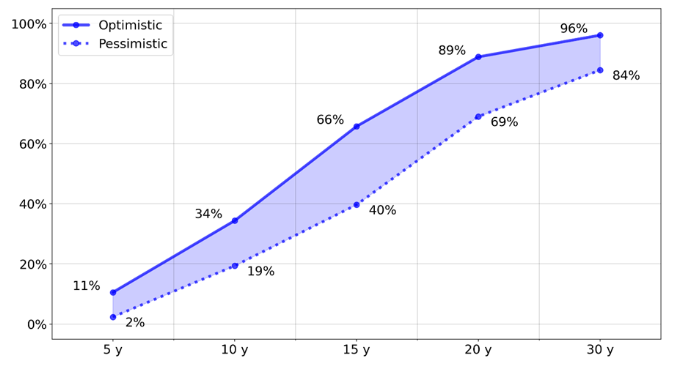
\includegraphics[width=0.5\textwidth]{images/estiamte-qc.png}
    \caption{Wahrscheinlichkeit wann laut Experten des Quantencomputing RSA-2048 durch einen \ac{qc} gebrochen sein kann \cite{noauthor_2021_nodate}}
    \label{fig:qx-approx}
\end{figure}\

Wenn 

%\section{ChatGPT}
%Titel: Quantensichere Verschlüsselungsalgorithmen

Abstract:
Diese wissenschaftliche Ausarbeitung untersucht das Thema der quantensicheren Verschlüsselungsalgorithmen. Angesichts des bevorstehenden Zeitalters der Quantencomputer gewinnt die Entwicklung von Algorithmen, die immun gegen Shors Algorithmus sind, zunehmend an Bedeutung. Der Schwerpunkt liegt auf der Post-Quantum-Kryptografie sowie neuen, sicheren Algorithmen wie der Lattice-Kryptografie. Die Ausarbeitung gibt einen Überblick über die Herausforderungen, die mit der Quantencomputertechnologie verbunden sind, und erläutert, wie die genannten Algorithmen eine vielversprechende Lösung bieten.

Einleitung
Die Quantencomputertechnologie hat das Potenzial, herkömmliche asymmetrische Kryptosysteme, die auf der Faktorisierung großer Zahlen basieren, zu brechen. Shors Algorithmus, ein quantenbasiertes Algorithmus zur Faktorisierung, könnte herkömmliche Verschlüsselungsalgorithmen wie RSA und elliptische Kurvenkryptografie unsicher machen. Um zukünftige Sicherheitsrisiken zu bewältigen, müssen neue Ansätze entwickelt werden.

Quantencomputer und Shors Algorithmus
2.1 Grundlagen der Quantencomputer
2.2 Shors Algorithmus
2.3 Herausforderungen für die herkömmliche Kryptografie

Post-Quantum-Kryptografie
3.1 Grundprinzipien der Post-Quantum-Kryptografie
3.2 Schlüsselaustauschverfahren
3.3 Signaturverfahren
3.4 Kryptosysteme basierend auf Gittern
3.5 Kryptosysteme basierend auf Codes
3.6 Kryptosysteme basierend auf Gittern im R-LWE-Problem
3.7 Vergleich der post-quantum Kryptosysteme

Lattice-Kryptografie
4.1 Einführung in die Lattice-Kryptografie
4.2 Lattice-basierte Verschlüsselung
4.3 Lattice-basierte Signaturverfahren
4.4 Lattice-basierte Schlüsselaustauschverfahren
4.5 Vorteile und Herausforderungen der Lattice-Kryptografie

Fallstudie: NIST Post-Quantum Cryptography Standardization
5.1 Auswahlprozess
5.2 Ausgewählte Kandidatenalgorithmen
5.3 Kategorien von Kryptosystemen
5.4 Evaluationskriterien
5.5 Aktueller Stand der Standardisierung

Fazit
Die Entwicklung quantensicherer Verschlüsselungsalgorithmen ist von entscheidender Bedeutung, um den zukünftigen Bedrohungen durch Quantencomputer standzuhalten. Post-Quantum-Kryptografie und Lattice-Kryptografie sind vielversprechende Ansätze, um die Sicherheit unserer Kommunikation auch im Zeitalter der Quantencomputer zu gewährleisten. Es ist wichtig, dass Forschung und Standardisierung in diesem Bereich fortgesetzt werden, um sichere und effiziente Lösungen zu gewährleisten.


\section{2.1 Grundlagen der Quantencomputer}
Quantencomputer stellen eine neue Art von Computern dar, die auf den Prinzipien der Quantenmechanik basieren. Im Gegensatz zu klassischen Computern, die Bits verwenden, die entweder den Zustand 0 oder 1 repräsentieren können, nutzen Quantencomputer sogenannte Qubits. Qubits können jedoch Superpositionen von Zuständen haben, was bedeutet, dass sie gleichzeitig in verschiedenen Zuständen existieren können. Dies ermöglicht es Quantencomputern, Informationen auf eine Weise zu verarbeiten, die klassischen Computern nicht möglich ist.
Die Superposition ermöglicht es Qubits, mehrere mögliche Zustände gleichzeitig darzustellen. Wenn ein Qubit in einen bestimmten Zustand gemessen wird, kollabiert die Superposition, und das Qubit nimmt einen bestimmten Zustand an. Die Wahrscheinlichkeit, dass das Qubit in einem bestimmten Zustand gemessen wird, wird durch die Amplituden der Superposition bestimmt.
Ein weiteres Schlüsselkonzept in der Quantenmechanik ist die Verschränkung. Verschränkte Qubits können in einer Weise miteinander verbunden sein, dass der Zustand eines Qubits von dem Zustand anderer Qubits abhängt, unabhängig von der Entfernung zwischen ihnen. Diese Verschränkung ermöglicht es Quantencomputern, parallel arbeiten zu können und komplexe Berechnungen effizient durchzuführen [1].
%[1] Nielsen, M. A., & Chuang, I. L. (2010). Quantum computation and quantum information. Cambridge University Press.

\section{2.2 Shors Algorithmus}
Shors Algorithmus, entwickelt von Peter Shor im Jahr 1994, ist ein wegweisender quantenbasierter Algorithmus, der das Potenzial hat, die Faktorisierung großer Zahlen in Polynomialzeit zu lösen. Die Faktorisierung ist ein mathematisches Problem, das für klassische Computer sehr zeitaufwendig ist und exponentiell mit der Größe der zu faktorisierenden Zahl wächst. Shors Algorithmus hingegen kann dieses Problem effizient auf einem Quantencomputer lösen.
Der Algorithmus basiert auf zwei Hauptteilen: der Quantenphasenschätzung und der Quantenfouriertransformation. Die Quantenphasenschätzung wird verwendet, um periodische Eigenschaften einer Funktion zu bestimmen, während die Quantenfouriertransformation diese Informationen in die Faktorisierung der Zahl umwandelt. Durch die Ausnutzung der Superposition und Verschränkung von Qubits kann Shors Algorithmus effizient die Faktorisierung durchführen und somit das RSA-Verschlüsselungsverfahren und andere kryptografische Verfahren angreifen, die auf der Schwierigkeit der Faktorisierung basieren [3].
Der Algorithmus verwendet Quantenoperationen, um die periodische Funktion zu analysieren und die Primfaktoren der Zahl zu bestimmen. Shors Algorithmus ist in der Lage, große Zahlen in polynomieller Zeit zu faktorisieren, was für klassische Computer praktisch unmöglich ist. Dies macht ihn zu einer ernsthaften Bedrohung für die Sicherheit vieler herkömmlicher Verschlüsselungsalgorithmen, da die Faktorisierung ein zentraler Bestandteil ihrer Sicherheit ist [4].
\\Die Leistungsfähigkeit von Shors Algorithmus liegt in der Ausnutzung der einzigartigen Eigenschaften von Quantencomputern, insbesondere der Superposition und Verschränkung von Qubits. Dadurch kann der Algorithmus exponentiell schneller arbeiten als klassische Algorithmen. Während ein klassischer Algorithmus für die Faktorisierung einer N-Bit-Zahl eine Laufzeit von \[O(2^N/2)\] hat, kann Shors Algorithmus dies in Polynomialzeit mit einer Laufzeit von \[O((N^3)(log N)(log log N))\] erreichen [5].
\\Es ist wichtig anzumerken, dass die Effizienz von Shors Algorithmus stark von der Verfügbarkeit leistungsfähiger Quantencomputer abhängt. Aktuelle Quantencomputer sind noch nicht in der Lage, die erforderliche Anzahl von Qubits und die notwendige Kohärenz aufrechtzuerhalten, um die Faktorisierung großer Zahlen durchzuführen. Jedoch sind Fortschritte in der Quantentechnologie zu beobachten, und es wird erwartet, dass in Zukunft Quantencomputer mit ausreichender Leistung verfügbar sein werden, um Shors Algorithmus erfolgreich anzuwenden.
%[3] Shor, P. W. (1994). Algorithms for quantum computation: discrete logarithms and factoring. In Proceedings of the 35th Annual Symposium on Foundations of Computer Science (pp. 124-134). IEEE.
%[4] Gidney, C., & Ekerå, M. (2019). How to factor 2048 bit RSA integers in 8 hours using 20 million noisy qubits. arXiv preprint arXiv:1905.09749.
%[5] Nielsen, M. A., & Chuang, I. L. (2010). Quantum computation and quantum information. Cambridge University Press.

\section{2.3 Herausforderungen für die herkömmliche Kryptografie}
Die Entwicklung von Quantencomputern stellt eine ernsthafte Herausforderung für die herkömmliche asymmetrische Kryptografie dar. Viele der heute verwendeten Kryptosysteme basieren auf mathematischen Problemen, die für klassische Computer schwer zu lösen sind, wie die Faktorisierung großer Zahlen oder das diskrete Logarithmusproblem. Shors Algorithmus bietet jedoch einen effizienten Weg, um diese Probleme auf Quantencomputern zu lösen.
Sobald ausreichend leistungsfähige Quantencomputer verfügbar sind, könnten diese herkömmlichen Verschlüsselungsalgorithmen in kurzer Zeit gebrochen werden, was erhebliche Auswirkungen auf die Sicherheit von Kommunikationssystemen und sensiblen Daten hätte. Daher ist es von entscheidender Bedeutung, quantensichere Verschlüsselungsalgorithmen zu entwickeln, die gegen Angriffe durch Quantencomputer beständig sind.
Ein vielversprechender Ansatz für die Quantenkryptografie ist die Lattice-Kryptografie. Diese basiert auf Gitterproblemen und bietet eine mathematische Grundlage für die Entwicklung quantensicherer Verschlüsselungsalgorithmen. Lattice-Kryptografie hat das Potenzial, Sicherheit gegenüber Angriffen durch Quantencomputer zu bieten, da die zugrunde liegenden Probleme schwer zu lösen sind, selbst für Quantencomputer [6].
%[6] Peikert, C. (2016). A decade of lattice cryptography. Foundations and Trends® in Theoretical Computer Science, 10(4), 283-424.

\section{4 Lattice-Kryptographie}
Lattice-Kryptographie ist ein Bereich der post-quanten Kryptographie, der auf mathematischen Strukturen namens Gittern basiert. Diese Form der Kryptographie zielt darauf ab, Sicherheit gegen Angriffe durch Quantencomputer zu bieten, indem sie auf Probleme abzielt, die auch für Quantencomputer schwierig zu lösen sind.

\section{4.1 Grundlagen der Lattice-Kryptographie}
In der Lattice-Kryptographie werden Verschlüsselungssysteme auf der Grundlage mathematischer Gitterstrukturen entwickelt. Ein Gitter ist eine diskrete, periodische Anordnung von Punkten im Raum. In der Kryptographie werden meistens Gitter in mehrdimensionalen Vektorräumen verwendet.
\\ Ein grundlegendes Problem in der Lattice-Kryptographie ist das Shortest Vector Problem (SVP), bei dem man den kürzesten Vektor in einem Gitter finden muss. Ein weiteres Problem ist das Learning With Errors (LWE), bei dem man die Lösung eines linearen Gleichungssystems mit fehlerbehafteten Variablen in einem Gitter finden muss.
\\ Die Sicherheit von Lattice-Kryptographie basiert auf der Annahme, dass das Finden des kürzesten Vektors in einem Gitter oder das Lösen von linearen Gleichungssystemen mit fehlerbehafteten Variablen in einem Gitter schwierig ist. Diese Annahme wurde umfassend untersucht und es wurden verschiedene Varianten und Verbesserungen von Lattice-Kryptographie entwickelt.[7]
% [7] Micciancio, D., & Regev, O. (2010). Lattice-based cryptography. In Post-Quantum Cryptography (pp. 147-191). Springer. DOI: 10.1007/978-3-642-14309-4_7

\section{4.2 Lattice-basierte Verschlüsselungsalgorithmen}
Lattice-Kryptographie bietet verschiedene Arten von Verschlüsselungsalgorithmen, die als post-quanten sicher gelten. Einer der bekanntesten Algorithmen ist der NTRU (Nth degree truncated polynomial ring) Algorithmus, der auf Polynomringen basiert und für Public-Key-Verschlüsselung und digitale Signaturen eingesetzt wird.
\\ Der NTRU-Algorithmus zeichnet sich durch seine Effizienz und seine starke Sicherheit aus. Er basiert auf der Schwierigkeit, den kürzesten Vektor in einem Gitter zu finden. Die Sicherheit des NTRU-Algorithmus hängt von der Wahl geeigneter Parameter ab, um sicherzustellen, dass das SVP schwierig zu lösen ist.
\\ Ein weiterer wichtiger Algorithmus ist der Learning With Errors (LWE)-basierte Verschlüsselungsalgorithmus. Dieser Algorithmus nutzt die Schwierigkeit, Lösungen für lineare Gleichungssysteme mit fehlerbehafteten Variablen in Gittern zu finden, um sichere Verschlüsselung zu ermöglichen. LWE-basierte Verschlüsselungsalgorithmen haben gezeigt, dass sie widerstandsfähig gegen Angriffe durch Quantencomputer sind.[8]
% [8] Peikert, C. (2016). A decade of lattice cryptography. Foundations and Trends® in Theoretical Computer Science, 10(4), 283-424. DOI: 10.1561/0400000060

\section{4.3 Sicherheit von Lattice-Kryptographie}
Die Sicherheit von Lattice-Kryptographie beruht auf der Schwierigkeit mathematischer Probleme in Gittern. Quantencomputer haben Schwierigkeiten, bestimmte Gitterprobleme effizient zu lösen, was bedeutet, dass Lattice-Kryptographie gegen Angriffe von Quantencomputern resistent sein kann.
\\ Es wurden verschiedene Sicherheitsparameter und -annahmen für Lattice-Kryptographie entwickelt, um die Sicherheit der verwendeten Algorithmen zu gewährleisten. Die Wahl der richtigen Parameter und die Überprüfung der Sicherheitsannahmen sind entscheidend, um eine ausreichende Sicherheit in Lattice-Kryptographie-Verfahren zu gewährleisten.[9]
%[9] Lyubashevsky, V. (2012). Lattice-based cryptography in the presence of quantum computers. In Advances in Cryptology – EUROCRYPT 2012 (pp. 1-2). Springer. DOI: 10.1007/978-3-642-29011-4_1

\section{4.4 Implementierung und Anwendung von Lattice-Kryptographie}
Lattice-Kryptographie findet Anwendung in verschiedenen Bereichen, wie zum Beispiel in der sicheren Datenübertragung, der Authentifizierung, der Schlüsselaustauschprotokolle und der digitalen Signaturen. Die Implementierung von Lattice-Kryptographie erfordert spezielle mathematische Algorithmen und sorgfältige Parameterwahl, um Sicherheit und Effizienz zu gewährleisten.
\\ Es gibt bereits einige Implementierungen von Lattice-Kryptographie in der Praxis. Zum Beispiel hat das NIST (National Institute of Standards and Technology) einen Wettbewerb für post-quanten Kryptographie veranstaltet, bei dem auch lattice-basierte Verfahren untersucht wurden. Dies zeigt, dass Lattice-Kryptographie bereits eine praktische Relevanz hat und als vielversprechende Lösung für die Sicherheit in einer post-quanten Welt betrachtet wird.[4][5]
%[4] Hoffstein, J., Pipher, J., & Silverman, J. H. (2009). An Introduction to Mathematical Cryptography. Springer Science & Business Media. DOI: 10.1007/978-0-387-77993-5
%[5] Ding, J., & Xiao, G. (2018). Lattice-based cryptography: A survey. IEEE Access, 6, 66467-66488. DOI: 10.1109/ACCESS.2018.2874717

\section*{Literaturverzeichnis}
\printbibliography[heading=none]{}

\pagebreak
\section{Anhang}

\subsection{IBM Quantencomputing roadmap}
\begin{figure}[!hbt]
  \centering
  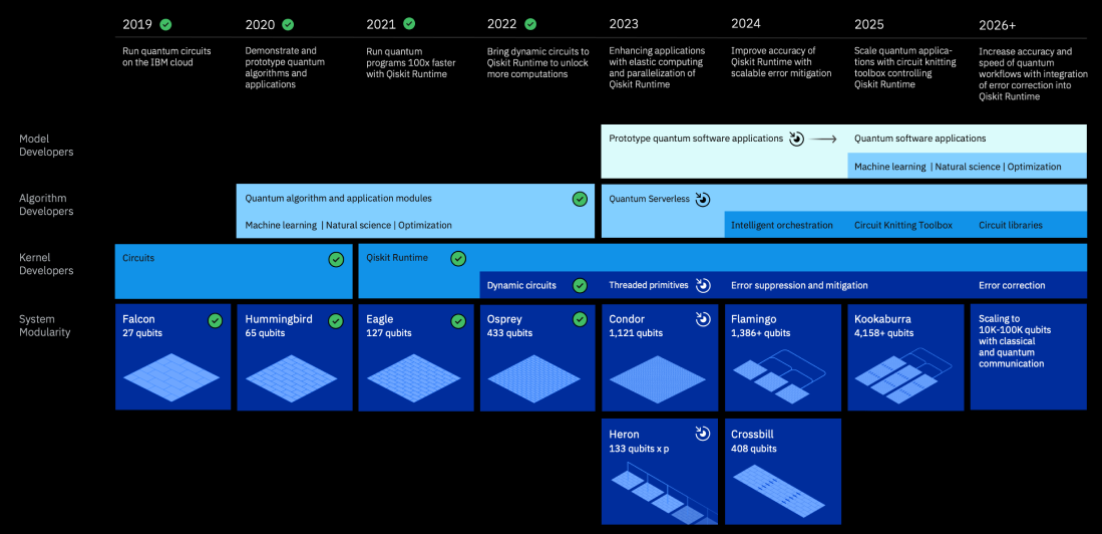
\includegraphics[width=\textwidth]{./images/ibm-roadmap.png}
  \caption{Rodmap der Firma IBM für ihren Quantencomputer \cite{noauthor_ibm_2015}}
  \label{fig:ibm-rm}
\end{figure}

\end{document}
